%% FEUP THESIS STYLE for LaTeX2e
%% how to use feupteses (portuguese version)
%%
%% FEUP, JCL & JCF, 31 Jul 2012
%%
%% PLEASE send improvements to jlopes at fe.up.pt and to jcf at fe.up.pt
%%

%%========================================
%% Commands: pdflatex tese
%%           bibtex tese
%%           makeindex tese (only if creating an index)
%%           pdflatex tese
%% Alternative:
%%          latexmk -pdf tese.tex
%%========================================

%% 2021-07-20: One-sided output by default
\documentclass[11pt,a4paper]{report}
%% For two-sided printing (for dead-tree output) comment previous line
%% and uncomment the next line
%% \documentclass[11pt,a4paper,twoside,openright]{report}

%% For iso-8859-1 (latin1), comment next line and uncomment the second line
\usepackage[utf8]{inputenc}
%\usepackage[latin1]{inputenc}

%% Portuguese version

%% MEIC options
%\usepackage[portugues,meic]{feupteses}
%\usepackage[portugues,meic,juri]{feupteses}
%\usepackage[portugues,meic,final]{feupteses}
%\usepackage[portugues,meic,final,onpaper]{feupteses}

%% MEEC options
%\usepackage[portugues,meec]{feupteses}
%\usepackage[portugues,meec,juri]{feupteses}
%\usepackage[portugues,meec,final]{feupteses}
%\usepackage[portugues,meec,final,onpaper]{feupteses}

%% For other degrees
\usepackage[portugues]{feupteses} % you must define the degree bellow

%% Options: 
%% - portugues: titles, etc in portuguese
%% - onpaper: links are not shown (for paper versions)
%% - backrefs: include back references from bibliography to citation place

%% Uncomment to create an index (at the end of the document)
%\makeindex

%% Path to the figures directory
%% TIP: use folder ``figures'' to keep all your figures
\graphicspath{{figures/}}

%%----------------------------------------
%% TIP: if you want to define more macros, use an external file to keep them
%some macro definitions

% format
\newcommand{\class}[1]{{\normalfont\slshape #1\/}}

% entities
\newcommand{\Feup}{Faculdade de Engenharia da Universidade do Porto}

\newcommand{\svg}{\class{SVG}}
\newcommand{\scada}{\class{SCADA}}
\newcommand{\scadadms}{\class{SCADA/DMS}}

%%----------------------------------------

%%========================================
%% Start of document
%%========================================
\begin{document}

%%----------------------------------------
%% Information about the work
%%----------------------------------------
\title{Título da Dissertação}
\author{Nome do Autor}

%% Comment next line if not necessary for degree name
\degree{Programa Doutoral em Engenharia Informática}

%% Uncomment next line for date of submission
%\thesisdate{31 de julho de 2008}

%% Comment next line for copyright text if not used
\copyrightnotice{Nome do Autor, 2008}

\supervisor{Orientador}{Nome do Orientador}

%% Uncomment next line if necessary
%\supervisor{Co-orientador}{Nome de Outro Orientador}

%% Uncomment committee stuff in the final version if used
%\committeetext{Aprovado em provas públicas pelo Júri:}
%\committeemember{Presidente}{Nome do presidente do júri}
%\committeemember{Arguente}{Nome do arguente do júri}
%\committeemember{Vogal}{Nome do vogal do júri}

%% Uncomment signature line in the final on paper version if used
%\signature

%% Specify cover logo (in folder ``figures'')
\logo{uporto-feup.pdf}
 
%% Uncomment next line for additional text below the author's name (front page)
%\additionalfronttext{Preparação da Dissertação}

%%----------------------------------------
%% Preliminary materials
%%----------------------------------------

% remove unnecessary \include{} commands
\begin{Prolog}
  \chapter*{Abstract}
Machine learning (ML) models can perform a vast amount of tasks. Recognition of images and speech, statistical arbitrage (useful in finance), performing medical diagnostics through the analysis of medical exams, and performing predictive analysis are skills in their repertoire. The ML models must be trained using extensive data to accomplish these tasks.

%Each machine learning model needs to absorb data related to the task it will end up performing, 
Valid data is usually either scarce, expensive, or not readily available. Scrapping tools are commonly used to circumvent the scarceness of data, but their quality is questionable. A small dataset is also insufficient to produce an accurate prediction model. Even in cases where a large amount of data is available, its use may infringe privacy policies (a common problem when entering the medical field). These problems represent an accumulation of problematic data that leads to incorrect results. Synthetic datasets have a proven track record of improving ML effectiveness by providing a better dataset with fewer data imbalances than its "organic" bredren. 

The work developed in this study focus on the study of meta feature extraction methods and meta feature insertion analysis. Using an already existing Ticket-based Synthetic DataSet Generator as a basis, we also developed a meta extractor feature.

Each dataset has its group of meta features - its fingerprint. Our meta feature extractor feature can dissect any kind of CSV tabular dataset, even if those datasets were not synthetically generated by our generator.
%When an existing dataset is available, the generator should analyse it and its meta features extracted, then used as parameters for the generation process. This generation should also be available if no original dataset is provided by making a simple selection of parameters. 
Despite being referenced in many studies, meta features are not uniformly described. Nevertheless, some studies agree on lists of meta features, and those arranged lists are explored. Besides extracting parameters from existing datasets' meta features, it is also essential to analyse the parameter-parameter relationship.
%The quality of the synthetic dataset is also a factor of concern: cases of missing data, imbalances, anomalies and overfitting can easily happen during the generation process, and as such, the number of outliers must be realistic. Outliers should exist in a dataset as they contain useful information.

We also explored the concept of meta feature inclusion in the generation process, where we try to force values of certain meta features into the final synthetic dataset.

%The workflow started with the analysis and definition of a set of meta features, passing to the creation of parameters in the generator corresponding to that same data features. The quality assurance process will be the final step in the practical development of this study.

\vspace*{10mm}\noindent
\textbf{Keywords}: Synthetic Dataset, Meta Features, Machine Learning
 % the abstract
  \chapter*{Agradecimentos \footnote{Unlike the rest of this study, the acknowledgements are written in Portuguese to be read by every person mentioned, some of which are native only speakers.}}

Um trabalho de mestrado é uma longa caminhada, marcada por diversos desafios, incertezas, alegrias e tristezas. Apesar do processo solitário a que qualquer investigador está destinado, o seu percurso é também pautado pelo apoio de várias pessoas, às quais dedico este trabalho. 

Em primeiro lugar, gostaria de exprimir os mais sinceros agradecimentos ao meu orientador, professor doutor Daniel Castro Silva e ao meu co-orientador, Leonardo Silva Ferreira, pela orientação exemplar, rigor científico, disponibilidade e conselhos facultados ao longo dos últimos meses. 

Agradeço aos meus grandes amigos e colegas de curso, Ricardo Figueiredo e Luís Guilherme Neves, por terem sempre puxado por mim e me terem ajudado quando mais precisei – é também graças a vocês que este trabalho é possível. 

Obrigado aos meus amigos Sérgio Pinto, Rahul Pires, João Brandão, João Pedro Morais, Mafalda Neves, Inês Faria e Sara Aguiar por todos os momentos passados e amizade transmitida.  

Um obrigado à Tuna de Engenharia da Universidade do Porto (TEUP) - lugar onde encontrei a minha casa longe de casa, e por ter sido a escola que fez de mim grande parte da pessoa que sou hoje. 

Agradeço à minha terapeuta Dra. Sara Malheiro, pela atenção, disponibilidade, prontidão e amizade que me permitiram trilhar o caminho certo para aqui chegar. 

Ao professor doutor António Augusto Sousa, pelas constantes palavras de encorajamento e por uma conversa especial que fez com que fosse capaz de olhar para este percurso com outros olhos. 

Por fim, e como não podia deixar de ser, dirijo os meus maiores agradecimentos à minha família, que revelou ser o maior porto de abrigo e refúgio nos momentos mais difíceis.  

Aos meus pais, que sempre foram um exemplo de dedicação, trabalho e esforço. 

Ao meu irmão Pedro, meu melhor amigo, com quem partilho memórias e momentos muito felizes.  

Às minhas tias Helena e Elsa, que ao longo da vida (em especial dos anos no Porto) foram sempre a principal rede de apoio e ajuda para tudo, e a quem serei eternamente grato.  

Às minhas tias São, Zeza, e à minha prima Xana pelo carinho e amizade desde sempre.  

À Mariana, um especial e muito grande agradecimento por, mesmo nos momentos mais difíceis, nunca me ter deixado desistir e ter acreditado que tudo isto seria possível. Obrigado pelo carinho, dedicação e amor ao longo dos últimos nove anos.  
\vspace{10mm}
\flushleft{João Carlos Lemos}
  % the acknowledgments
  \cleardoublepage
\thispagestyle{plain}

\vspace*{8cm}

\begin{flushright}
  \textsl{“The story so far:\\
In the beginning the Universe was created.\\
This has made a lot of people very angry and been widely regarded as a bad move.”}\\
\vspace*{1.5cm}
    Douglas Adams, The Restaurant at the End of the Universe
\end{flushright}
    % initial quotation if desired
  \cleardoublepage
  \pdfbookmark[0]{Conteúdo}{contents}
  \tableofcontents
  \cleardoublepage
  \pdfbookmark[0]{Lista de Figuras}{figures}
  \listoffigures
  \cleardoublepage
  \pdfbookmark[0]{Lista de Tabelas}{tables}
  \listoftables
  \chapter*{Abbreviations}
\chaptermark{ABBREVIATIONS}
%\chapter*{Acrónimos}
%\chaptermark{ACRONIMOS}


\begin{flushleft}
\begin{tabular}{l p{0.8\linewidth}}
DT & Decision Tree\\
GUI & Graphical User Interface\\
ML  & Machine Learning\\
MLM & Machine Learning Model\\
PCA & Principal Component Analysis\\
PET & Privacy-enhancing technologies\\
SD & Synthetic Dataset\\
\end{tabular}
\end{flushleft}  % the list of abbreviations used
\end{Prolog}

%%----------------------------------------
%% Body
%%----------------------------------------

\StartBody

%% TIP: use a separate file for each chapter
\chapter{Introdução} \label{chap:intro}

Este documento ilustra o formato a usar em dissertações na \Feup.
São dados exemplos de margens, cabeçalhos, títulos, paginação, estilos
de índices, etc. 
São ainda dados exemplos de formatação de citações, figuras e tabelas,
equações, referências cruzadas, lista de referências e índices.
Este documento não pretende exemplificar conteúdos a usar.

Uma recolha sobre as normas existentes pode ser encontrada em~\citet{kn:Mat93}.

Neste primeiro capítulo ilustra-se a utilização de citações e de
referências bibliográficas.

\section{Secção Exemplo} \label{sec:context}

Para além de dar um exemplo de utilização de uma citação, o parágrafo
seguinte introduz uma referência que pode ser consultada, entre muitas
outras referências bibliográficas interessantes~\citep{kn:Tha01,kn:PP05}.

\begin{quote}
  ``Like the Abstract, the Introduction should be written to engage the
  interest of the reader. It should also give the reader an idea of
  how the dissertation is structured, and in doing so, define the
  thread of the contents.''~\citep[chap.\ Introduction]{kn:Tha01} 
\end{quote}

Lorem ipsum~\citep{kn:Lip08} dolor sit amet, consectetuer adipiscing
elit. 
Sed eget nunc. Phasellus interdum, risus viverra mollis laoreet, felis
justo iaculis ante, eget ornare purus augue non urna. Nam in magna. In a
est. Phasellus a tellus vitae enim vehicula imperdiet. Etiam sit amet
elit. In hac habitasse platea dictumst. Quisque eget turpis vel felis
elementum tempus. Curabitur sit amet tortor id libero dapibus
pretium. Integer mattis eros eu lorem. Duis erat tellus, porttitor
sed, blandit eget, fringilla et, lacus. Phasellus tristique nibh nec
orci. Mauris sed leo. Suspendisse fringilla tempor dolor. Donec sapien
enim, congue in, porta et, sollicitudin in, quam. Curabitur semper,
mauris ut vestibulum eleifend, diam ipsum tincidunt quam, et
vestibulum velit mauris ut risus. 

Sed eget libero. Nulla facilisi. Proin eget tortor. Morbi
gravida. Donec arcu risus, blandit a, rutrum at, ornare ut,
nisl. Etiam consectetuer tortor eu odio. Etiam blandit molestie
ligula. Nulla facilisi. Nam a augue non justo laoreet hendrerit. Nam
aliquam, purus eu ultricies dictum, urna purus posuere neque, vel
tempus tellus enim a arcu. 

Pellentesque congue sapien in ligula. Nulla nec mi sed augue congue
tristique. Cras pretium. Pellentesque lobortis, libero id adipiscing
auctor, orci massa vehicula nulla, vel ullamcorper tortor ipsum ut
elit. Morbi rhoncus, dui sed tristique volutpat, lorem felis euismod
lorem, vel tristique nibh arcu vel eros. Nunc tempor. Sed et erat a
tortor fermentum consequat. Cras varius nisl accumsan libero. Aliquam
faucibus, justo ut pharetra blandit, est nibh ultrices est, vel
facilisis quam lectus ut enim. Aliquam convallis, nibh non bibendum
pharetra, nisl velit lobortis orci, ac ultrices neque sem viverra
massa. Donec malesuada. Aliquam ligula. Fusce in nisl. Etiam lacinia
est quis velit. Maecenas massa. Maecenas sed pede. Nulla
sodales. Etiam vitae erat. Duis tristique sem sit amet libero. Ut a
libero nec ligula tempus mattis. 

\section{Outra Secção Exemplo} \label{sec:goals}

Lorem ipsum dolor sit amet, consectetuer adipiscing elit. Morbi sit
amet nibh. Fusce faucibus, enim vel ultrices ornare, est mauris
ultricies velit, vitae consequat sem erat vel nunc. Nam libero eros,
mattis eget, sagittis nec, imperdiet at, sapien. Aliquam lacus. Aenean
adipiscing nibh in orci. Aliquam vestibulum, elit at fringilla
dignissim, metus diam lobortis urna, a laoreet nunc odio ac ipsum. Sed
at urna. Integer vehicula fringilla augue. Nulla lacus eros, rhoncus
sit amet, posuere ut, vehicula ac, nibh. Ut eleifend, eros eu placerat
vehicula, justo turpis blandit dolor, eu tincidunt felis risus at
ante. Aenean suscipit nisl eget eros. Ut laoreet libero eget
enim. Cras tempus pellentesque felis. Vestibulum vitae erat ac nibh
posuere eleifend. 

Integer nec quam. Sed fermentum. Nunc vitae leo. Etiam sit amet
quam. Nunc vestibulum massa in mauris. Duis eget nulla. Fusce
ultricies arcu eu nibh volutpat feugiat. Maecenas urna pede, commodo
quis, porta eu, bibendum elementum, pede. Sed eros massa, molestie
eget, mattis non, rutrum ac, magna. Duis dui. Maecenas eget tortor ut
dolor semper mattis. Maecenas auctor, tellus et ultricies tempor, elit
est placerat lacus, in posuere mauris lorem et arcu. 

Nulla nec eros et pede vehicula aliquam. Aenean sodales pede vel
ante. Fusce sollicitudin sodales lacus. Maecenas justo mauris,
adipiscing vitae, ornare quis, convallis nec, eros. Etiam laoreet
venenatis ipsum. In tellus odio, eleifend ac, ultrices vel, lobortis
sed, nibh. Fusce nunc augue, dictum non, pulvinar sed, consectetuer
eu, ipsum. Vivamus nec pede. Pellentesque pulvinar fringilla dolor. In
sit amet pede. Proin orci justo, semper vel, vulputate quis, convallis
ac, nulla. Nulla at justo. Mauris feugiat dolor. Etiam posuere
fermentum eros. Morbi nisl ipsum, tempus id, ornare quis, mattis id,
dolor. Aenean molestie metus suscipit dolor. Aliquam id lectus sed
nisl lobortis rhoncus. Curabitur vitae diam sed sem aliquet
tempus. Sed scelerisque nisi nec sem. 


\section{Estrutura da Dissertação} \label{sec:struct}

Para além da introdução, esta dissertação contém mais x capítulos.
No Capítulo~\ref{chap:sota}, é descrito o estado da arte e são
apresentados trabalhos relacionados. 
No Capítulo~\ref{chap:chap3}, ipsum dolor sit amet, consectetuer
adipiscing elit.
No Capítulo~\ref{chap:chap4} praesent sit amet sem. 
No Capítulo~\ref{chap:concl} posuere, ante non tristique
consectetuer, dui elit scelerisque augue, eu vehicula nibh nisi ac
est. 
 
\chapter{Revisão Bibliográfica} \label{chap:sota}

Neste capítulo é ilustrada a introdução de entradas no índice
remissivo e são feitas citações para a bibliografia.

Lorem ipsum dolor sit amet, consectetuer adipiscing elit. Donec a
eros. Phasellus non nulla non massa venenatis convallis. In
porta. Mauris quis magna. 

\section{Introdução}

Neste capítulo usa-se texto de um artigo apresentado na Conferência
XATA2006~\citep{kn:MVL06-xata}.

Nos últimos tempos têm surgido diversas soluções, apresentadas por
empresas do sector Auto\-ma\-ção de Sistemas para a disponibilização de
sistemas \scadadms{} na \textit{Web}.

Fusce risus mi, tristique eu, consectetuer id, auctor sed, elit. Donec
laoreet. Duis consectetuer interdum libero. Etiam eu orci. In eu
arcu. Fusce luctus diam eget lectus. Duis interdum lacus sed
ligula. Proin vestibulum felis eget lacus. Vivamus vestibulum, tellus
ut congue viverra, mauris lacus tempor turpis, eu congue nisi magna at
dolor. Ut molestie vehicula libero. Praesent in neque sed risus tempus
ornare. Donec hendrerit, erat eu semper aliquam, pede nulla dapibus
risus, ut pretium orci pede et neque.
Etiam eget tortor a metus convallis viverra. Quisque eget nisi sed
orci facilisis interdum. Aliquam non felis. 

\section{Secção Exemplo}\label{sec:dialecto}

\emph{Scalable Vector Graphics}\index{SVG}\index{XML!SVG} é uma
linguagem em formato XML que descreve gráficos de duas dimensões. 
Este formato padronizado pela W3C (\emph{World Wide Web Consortium})
é livre de patentes ou direitos de autor e está totalmente
documentado, à semelhança de outros W3C
standards~\citep{kn:svgdoc}.

Sendo uma linguagem XML, o \svg{} herda uma série de vantagens: a
possibilidade de transformar \svg{} usando técnicas como
XSLT\index{XML!XSLT}, de embeber \svg{} em qualquer documento
XML\index{XML} usando \textit{namespaces} ou até de  
estilizar \svg{} recorrendo a CSS\index{CSS} (\emph{Cascade Style Sheets}). 
De uma forma geral, pode dizer-se que \svg{}s interagem bem com as
atuais tecnologias ligadas ao XML e à Web, tal como referido
em~\citep{kn:svgibm,kn:svgw3c}.

Lorem ipsum dolor sit amet, consectetuer adipiscing elit. Donec a
eros. Phasellus non nulla non massa venenatis convallis. In
porta. Mauris quis magna. Proin mauris eros, aliquet id, eleifend
vitae, semper quis, erat. Aliquam id lectus non odio dignissim
blandit. Vestibulum porttitor arcu ut ligula. Nunc quis
erat. Curabitur ipsum tortor, ornare vitae, dapibus pretium, hendrerit
sed, urna. Vestibulum ante ipsum primis in faucibus orci luctus et
ultrices posuere cubilia Curae; Phasellus bibendum, nulla eget varius
aliquam, tortor nulla sollicitudin quam, vel vestibulum nisl magna at
sem. Aliquam velit sapien, ultrices viverra, tempus quis, ultrices at,
dui. Aliquam sit amet justo. Quisque tristique, metus eu iaculis
sagittis, urna leo bibendum diam, a ultricies sem diam a augue. Mauris
consectetuer, libero vel euismod tincidunt, nisi metus viverra ante,
quis pretium sapien odio nec risus. Nunc semper auctor
nulla\footnote{Exemplo de nota de rodapé.}. 

\subsection{Subsecção Exemplo} \label{batik} 

Batik é um conjunto de bibliotecas baseadas em \textit{Java} que
permitem o uso de imagens \svg{} (visualização, geração ou
manipulação) em aplicações ou \textit{applets}~\citep{kn:batik}.  
O projeto Batik\index{Batik} destina-se a fornecer ao programador
alguns módulos que permitem desenvolver soluções especificas usando
\svg~\citep{kn:svgdoc}. 

Lorem ipsum dolor sit amet, consectetuer adipiscing elit. Nunc eu
nulla. Pellentesque vitae nibh ultrices quam iaculis
convallis. Aliquam purus eros, varius eget, volutpat sodales,
imperdiet nec, lacus. Curabitur in elit sed sem rutrum posuere. Class
aptent taciti sociosqu ad litora torquent per conubia nostra, per
inceptos himenaeos. Duis sem. Praesent ultricies odio vel
sapien. Integer faucibus malesuada libero. Cras semper, dolor id
ullamcorper varius, magna risus volutpat felis, id pellentesque nulla
ante at erat. Integer sodales. 

Quisque sit amet odio. In at risus sit amet turpis interdum
posuere. Maecenas iaculis vehicula sem. Ut leo arcu, malesuada vel,
imperdiet id, dignissim a, purus. Duis eleifend, lectus non venenatis
dignissim, risus libero imperdiet mi, nec gravida massa libero sed
mauris. Nullam lobortis libero non sapien. Integer convallis iaculis
erat. Morbi dictum. Ut ultrices pellentesque velit. Cras ac
ante. Etiam in neque tincidunt lacus gravida vehicula. Proin et nisi. 

Vivamus non nunc nec risus tempor varius. Quisque bibendum mi at
dolor. Aliquam consectetuer condimentum risus. Aliquam luctus pulvinar
sem. Duis aliquam, urna et vulputate tristique, dui elit aliquet nibh,
vel dignissim magna turpis id sapien. Duis commodo sem id
quam. Phasellus dolor. Class aptent taciti sociosqu ad litora torquent
per conubia nostra, per inceptos himenaeos. 

\subsection{Subsecção Exemplo}

Loren ipsum dolor sit amet, consectetuer adipiscing elit. 
Praesent sit amet sem. Maecenas eleifend facilisis leo. Vestibulum et
mi. Aliquam posuere, ante non tristique consectetuer, dui elit
scelerisque augue, eu vehicula nibh nisi ac est. Suspendisse elementum
sodales felis. Nullam laoreet fermentum urna. 

Duis eget diam. In est justo, tristique in, lacinia vel, feugiat eget,
quam. Pellentesque habitant morbi tristique senectus et netus et
malesuada fames ac turpis egestas. Fusce feugiat, elit ac placerat
fermentum, augue nisl ultricies eros, id fringilla enim sapien eu
felis. Vestibulum ante ipsum primis in faucibus orci luctus et
ultrices posuere cubilia Curae; Sed dolor mi, porttitor quis,
condimentum sed, luctus in. 

\section{Resumo ou Conclusões}

Aliquam erat volutpat. Nunc pede ipsum, porttitor eu, bibendum non,
bibendum nec, nisl. Maecenas eget mauris. Nullam pulvinar. Curabitur
rutrum commodo est. Nam sapien pede, interdum eu, accumsan ultrices,
venenatis sit amet, tellus. Praesent ac ante bibendum enim varius
suscipit. Donec enim. Proin nisi. Quisque libero turpis, varius ut,
elementum vel, pulvinar sed, nunc. 

\chapter{Capítulo Exemplo}\label{chap:chap3}

Neste capítulo apresentam-se exemplos de formatação de figuras e
tabelas, equações e referências cruzadas.

Maecenas eleifend facilisis leo. Vestibulum et
mi. Aliquam posuere, ante non tristique consectetuer, dui elit
scelerisque augue, eu vehicula nibh nisi ac est. 
Suspendisse elementum sodales felis. Nullam laoreet fermentum urna. 

\section{Introdução}

Apresenta-se de seguida um exemplo de
equação\footnote{\url{https://en.wikipedia.org/wiki/Equation}},
completamente fora do contexto\footnote{\url{https://www.overleaf.com/learn/latex/Mathematical_expressions}}:

\begin{eqnarray}
CIF_1: \hspace*{5mm}F_0^j(a) &=& \frac{1}{2\pi \iota} \oint_{\gamma} \frac{F_0^j(z)}{z - a} dz\\
CIF_2: \hspace*{5mm}F_1^j(a) &=& \frac{1}{2\pi \iota} \oint_{\gamma} \frac{F_0^j(x)}{x - a} dx \label{eq:cif}
\end{eqnarray}

Na Equação~\ref{eq:cif} lorem ipsum dolor sit amet, consectetuer
adipiscing elit. Suspendisse tincidunt viverra elit. Donec tempus
vulputate mauris. Donec arcu. Vestibulum condimentum porta
justo. Curabitur ornare tincidunt lacus. Curabitur ac massa vel ante
tincidunt placerat. Cras vehicula semper elit. Curabitur gravida, est
a elementum suscipit, est eros ullamcorper quam, sed cursus velit
velit tempor neque. Duis tempor condimentum ante. Nam
sollicitudin. Vestibulum adipiscing, orci eu tempor dapibus, risus
sapien porta metus, et cursus leo metus eget nibh. 

Pellentesque rutrum, sapien at viverra facilisis, metus eros blandit
sem, quis dictum erat metus eget erat. Vivamus malesuada dapibus
nulla. Maecenas nec purus. Suspendisse auctor mattis augue. Phasellus
enim nisi, iaculis sit amet, pellentesque a, iaculis in, dui. Integer
risus. 

\section{Secção Exemplo}

A arquitectura do visualizador assenta sobre os seguintes conceitos
base~\citep{kn:ZPMD97}: 

\begin{itemize}
\item \textbf{Componentes} --- Suspendisse auctor mattis augue \emph{push};
\item \textbf{Praesent} --- Sit amet sem maecenas eleifend facilisis leo;
\item \textbf{Pellentesque} --- Habitant morbi tristique senectus et netus.
\end{itemize}

\subsection{Exemplo de Figura}

É apresentado na Figura~\ref{fig:arch} da página~\pageref{fig:arch} um
exemplo de figura flutuante que deverá ficar no topo da página.

\begin{figure}[t]
    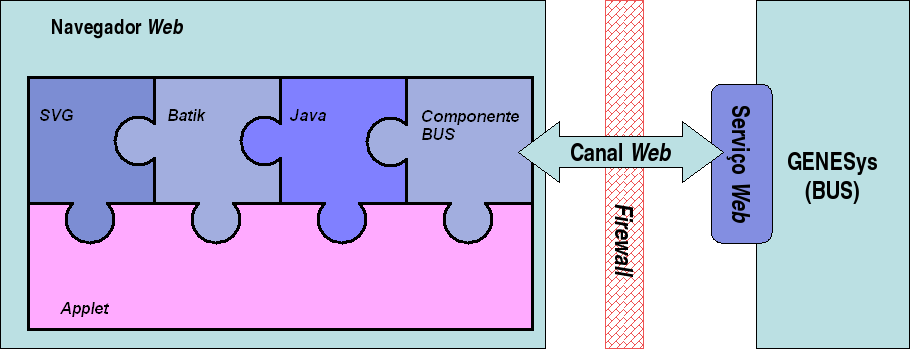
\includegraphics[width=0.86\textwidth]{puzzle}
    \caption{Arquitectura da Solução Proposta}
    \label{fig:arch}
\end{figure}

Loren ipsum dolor sit amet, consectetuer adipiscing elit. 
Praesent sit amet sem. Maecenas eleifend facilisis leo. Vestibulum et
mi. Aliquam posuere, ante non tristique consectetuer, dui elit
scelerisque augue, eu vehicula nibh nisi ac est. Suspendisse elementum
sodales felis. Nullam laoreet fermentum urna.

Duis eget diam. In est justo, tristique in, lacinia vel, feugiat eget,
quam. Pellentesque habitant morbi tristique senectus et netus et
malesuada fames ac turpis egestas. Fusce feugiat, elit ac placerat
fermentum, augue nisl ultricies eros, id fringilla enim sapien eu
felis. Vestibulum ante ipsum primis in faucibus orci luctus et
ultrices posuere cubilia Curae; Sed dolor mi, porttitor quis,
condimentum sed, luctus in. 

\subsection{Exemplo de Tabela}

É apresentado na Tabela~\ref{tab:exemplo} um exemplo de tabela
flutuante que deverá ficar no topo da página.

\begin{table}[t]
  \caption{Tabela Exemplo}
\begin{tabular}{|c|r@{.}lr@{.}lr@{.}l||r|}
	\hline
\multicolumn{8}{|c|}
	{\rule[-3mm]{0mm}{8mm}Iteração $k$ de $f(x_n)$} \\
\textbf{\em k}
	& \multicolumn{2}{c}{$x_1^k$}
	& \multicolumn{2}{c}{$x_2^k$}
	& \multicolumn{2}{c||}{$x_3^k$}
	& comentários \\ \hline \hline
0   & -0&3                 & 0&6                 &  0&7   & - \\
1   &  0&47102965 & 0&04883157 & -0&53345964  & $\delta<\epsilon$ \\
2   &  0&49988691 & 0&00228830 & -0&52246185  & $\delta < \varepsilon$ \\
3   &  0&49999976 & 0&00005380 & -0&523656   &   $N$ \\
4   &  0&5                 & 0&00000307 & -0&52359743  & \\
\vdots	& \multicolumn{2}{c}{\vdots}
	& \multicolumn{2}{c}{$\ddots$}
	& \multicolumn{2}{c||}{\vdots}  & \\
7   &  0&5   & 0&0    & \textbf{-0}&\textbf{52359878}
		 & $\delta<10^{-8}$ \\ \hline
\end{tabular}
  \label{tab:exemplo}
\end{table}

Loren ipsum dolor sit amet, consectetuer adipiscing elit. 
Praesent sit amet sem. Maecenas eleifend facilisis leo. Vestibulum et
mi. Aliquam posuere, ante non tristique consectetuer, dui elit
scelerisque augue, eu vehicula nibh nisi ac est. Suspendisse elementum
sodales felis. Nullam laoreet fermentum urna. 

Duis eget diam. In est justo, tristique in, lacinia vel, feugiat eget,
quam. Pellentesque habitant morbi tristique senectus et netus et
malesuada fames ac turpis egestas. Fusce feugiat, elit ac placerat
fermentum, augue nisl ultricies eros, id fringilla enim sapien eu
felis. Vestibulum ante ipsum primis in faucibus orci luctus et
ultrices posuere cubilia Curae; Sed dolor mi, porttitor quis,
condimentum sed, luctus in. 

\section{Secção Exemplo}

Loren ipsum dolor sit amet, consectetuer adipiscing elit. 
Praesent sit amet sem. Maecenas eleifend facilisis leo. Vestibulum et
mi. Aliquam posuere, ante non tristique consectetuer, dui elit
scelerisque augue, eu vehicula nibh nisi ac est. Suspendisse elementum
sodales felis. Nullam laoreet fermentum urna. 

\begin{lstlisting}[language=Python, caption=Python example]
# take the users input
words = input("Enter the text to translate to pig latin: ")
print(f"You entered: {words}")

# now, break apart the words into a list
words = words.split(' ')

# let's use the list to translate words greater than 3 characteres
for i in words:
    if len(i) >= 3:
        i = i + "%say" % (i[0])
        i = i[1:]
        print(i)
    else:
        pass
\end{lstlisting}

Duis eget diam. In est justo, tristique in, lacinia vel, feugiat eget,
quam. Pellentesque habitant morbi tristique senectus et netus et
malesuada fames ac turpis egestas. Fusce feugiat, elit ac placerat
fermentum, augue nisl ultricies eros, id fringilla enim sapien eu
felis. Vestibulum ante ipsum primis in faucibus orci luctus et
ultrices posuere cubilia Curae; Sed dolor mi, porttitor quis,
condimentum sed, luctus in.

\section{Resumo}

Pellentesque habitant morbi tristique senectus et netus et
malesuada fames ac turpis egestas. Fusce feugiat, elit ac placerat
fermentum, augue nisl ultricies eros, id fringilla enim sapien eu
felis. Vestibulum ante ipsum primis in faucibus orci luctus et
ultrices posuere cubilia Curae; Sed dolor mi, porttitor quis,
condimentum sed, luctus in. 

\chapter{Mais um Capítulo}\label{chap:chap4}

Neste capítulo mostra-se apenas o formato da dissertação.

Ipsum dolor sit amet, consectetuer
adipiscing elit.  Praesent sit amet sem. 
Maecenas eleifend facilisis leo. Vestibulum et
mi. Aliquam posuere, ante non tristique consectetuer, dui elit
scelerisque augue, eu vehicula nibh nisi ac est. 
Suspendisse elementum sodales felis. 
Nullam laoreet fermentum urna. 

\section{Secção Exemplo}

Lorem ipsum dolor sit amet, consectetuer adipiscing elit. Integer
hendrerit commodo ante. Pellentesque nibh libero, aliquam at, faucibus
id, commodo a, velit. Duis eleifend sem eget leo. Morbi in
est. Suspendisse magna sem, varius nec, hendrerit non, tincidunt quis,
quam. Aenean congue. Vivamus vel est sit amet sem iaculis
posuere. Cras mollis, enim vel gravida aliquam, libero nunc
ullamcorper dui, ullamcorper sodales lectus nulla sed urna. Morbi
aliquet porta risus. Proin vestibulum ligula a purus. Maecenas a
nulla. Maecenas mattis est vitae neque auctor tempus. Etiam nulla dui,
mattis vitae, porttitor sed, aliquet ut, enim. Cras nisl magna,
aliquet et, laoreet at, gravida ac, neque. Sed id est. Nulla dapibus
dolor quis ipsum rhoncus cursus. 

Etiam nisi est, dignissim sodales, fermentum id, pulvinar ac,
eros. Duis id orci. Nam pretium nisl ac augue. Ut adipiscing magna
eget est. Curabitur varius. Nulla facilisi. Pellentesque sit amet
neque ac dui accumsan blandit. Donec mauris felis, egestas sit amet,
convallis ac, dignissim quis, dolor. Maecenas cursus tortor vel
leo. Quisque tristique. Nunc augue odio, tincidunt in, dapibus sed,
ultricies sit amet, lorem. In hac habitasse platea dictumst. Praesent
iaculis, lacus hendrerit tempor sodales, libero tellus aliquet orci,
ut rhoncus massa lectus quis erat. Pellentesque quis dolor nec tortor
rhoncus convallis. Aliquam erat volutpat. Fusce placerat, magna eu
imperdiet lobortis, augue massa blandit turpis, a consectetuer quam
arcu sit amet risus. Suspendisse potenti. Praesent sapien metus,
interdum vitae, fermentum id, faucibus ut, lorem. Nunc iaculis purus
id tortor. Aenean risus pede, laoreet ac, tristique sed, lobortis in,
turpis (see Figure~\ref{fig:2figs-b}). 

\begin{figure}
  \subfloat[UP at the left]{\label{fig:2figs-a}
    {
\includegraphics[width=5cm]{uporto-feup}}
  }
  \qquad
  \subfloat[UP at the right]{\label{fig:2figs-b}
    {
\includegraphics[width=5cm]{uporto-feup}}
  }
  \caption{Two Figures side by side}
  \label{fig:2figs}
\end{figure}

Vestibulum et lorem in ligula viverra pharetra. Curabitur quis purus
in urna facilisis bibendum. Pellentesque at arcu accumsan velit
bibendum ornare. Praesent massa. Quisque dolor. In libero. Vestibulum
ac diam id leo feugiat blandit. Donec porta, tellus ac pellentesque
molestie, felis mauris viverra lacus, sed dignissim purus justo eu
justo. Proin iaculis, nunc eu volutpat volutpat, libero purus rutrum
enim, id euismod lacus lorem nec augue. Donec hendrerit lacinia
ante. Integer mollis vulputate orci. In pellentesque, metus pharetra
elementum pharetra, est purus bibendum turpis, eu pretium sapien
libero convallis odio. Cras sodales bibendum risus. Sed mattis nulla
non leo. Nulla nunc. Phasellus egestas sodales massa. Class aptent
taciti sociosqu ad litora torquent per conubia nostra, per inceptos
himenaeos. Pellentesque habitant morbi tristique senectus et netus et
malesuada fames ac turpis egestas. Etiam mi. 

\section{Mais uma Secção}

Lorem ipsum dolor sit amet, consectetuer adipiscing elit. Quisque
purus sapien, interdum ut, vestibulum a, accumsan ullamcorper,
erat. Mauris a magna ut leo porta imperdiet. Donec dui odio, porta in,
pretium non, semper quis, orci. Quisque erat diam, pharetra vel,
laoreet ac, hendrerit vel, enim. Donec tristique luctus risus. Fusce
dolor est, eleifend id, elementum sit amet, varius vitae, neque. Morbi
at augue. Ut sem ligula, auctor vitae, facilisis id, pharetra non,
lectus. Nulla lacus augue, aliquam eget, sollicitudin sed, hendrerit
eu, leo. Suspendisse ac tortor. Mauris at odio. Etiam vehicula. Nam
lacinia purus at nibh. Aliquam fringilla lorem ac justo. Ut nec
enim. Nunc ornare, eros eu facilisis tristique, nisl lorem lacinia
risus, non ullamcorper tellus urna et eros. Quisque eleifend tempus
metus. Nunc ipsum. 

Phasellus ullamcorper justo id risus. Nunc in leo. Mauris auctor
lectus vitae est lacinia egestas. Nulla faucibus erat sit amet lectus
varius semper. Praesent ultrices vehicula orci. Nam at metus. Aenean
eget lorem nec purus feugiat molestie. Phasellus fringilla nulla ac
risus. Aliquam elementum aliquam velit. Aenean nunc odio, lobortis id,
dictum et, rutrum ac, ipsum. Aenean tellus magna, lacinia eget,
bibendum ut, interdum sit amet, ipsum. Class aptent taciti sociosqu ad
litora torquent per conubia nostra, per inceptos himenaeos. Mauris
felis lacus, dapibus sit amet, pretium feugiat, aliquet non,
purus. Aliquam elementum, diam quis porttitor gravida, sem sapien
iaculis nulla, ut pharetra odio felis a metus. Nulla lacus ipsum,
tristique ut, dapibus sed, mollis et, justo. Vivamus non ipsum sed
ligula placerat ultrices. Maecenas dictum leo adipiscing
mauris. Vestibulum tristique, lacus a consequat suscipit, nunc dui
sollicitudin arcu, non interdum libero est eget tortor. Ut eget neque
quis leo tempor dictum. 

Quisque ullamcorper. Aliquam vel magna. Sed pulvinar dictum
ligula. Sed ultrices dolor ut turpis. Vivamus sagittis orci malesuada
arcu venenatis auctor. Proin vehicula pharetra urna. Aliquam egestas
nunc quis nisl. Donec ullamcorper. Nulla purus. Ut suscipit lacus
vitae dui. Mauris semper. Ut eget sem. Integer orci. Nam vitae dui
eget nisi placerat convallis. 

Sed id lorem. Proin gravida bibendum lacus. Sed molestie, urna quis
euismod laoreet, diam dolor dictum diam, vitae consectetuer leo ipsum
id ante. Integer eu lectus non mauris pharetra viverra. In feugiat
libero ut massa. Morbi cursus, lorem sollicitudin blandit semper,
felis magna pellentesque lacus, ut rhoncus leo neque at tellus. Sed
mattis, diam eget eleifend tincidunt, ligula eros tincidunt diam,
vitae auctor turpis est vel nunc. In eu magna. Donec dolor metus,
egestas sit amet, ultrices in, faucibus sed, lectus. Etiam est enim,
vehicula pharetra, porta non, viverra vel, nunc. Ut non sem. Etiam nec
neque. Sed rhoncus, justo id imperdiet pharetra, mi tellus accumsan
neque, vitae volutpat tortor enim in odio. Nunc porta justo a
lorem. Nulla hendrerit odio vitae dolor. Suspendisse eu nisl.  

\section{Resumo ou Conclusões}

Proin vehicula pharetra urna. Aliquam egestas
nunc quis nisl. Donec ullamcorper. Nulla purus. Ut suscipit lacus
vitae dui. Mauris semper. Ut eget sem. Integer orci. Nam vitae dui
eget nisi placerat convallis. 

\chapter{Conclusões e Trabalho Futuro} \label{chap:concl}

Proin sed justo eu sapien eleifend elementum. Pellentesque
habitant morbi tristique senectus et netus et malesuada fames ac
turpis egestas. Vivamus quam lacus, pharetra vel, aliquam vel,
volutpat sed, nisl. 

\section{Satisfação dos Objetivos}

Lorem ipsum dolor sit amet, consectetuer adipiscing elit. Etiam non
felis sed odio rutrum ultrices. Donec tempor dolor. Vivamus justo
neque, tempus id, ullamcorper in, pharetra non, tellus. Praesent eu
orci eu dolor congue gravida. Sed eu est. Donec pulvinar, lectus et
eleifend volutpat, diam sapien sollicitudin arcu, a sagittis libero
neque et dolor. Nam ligula. Cras tincidunt lectus quis nunc. Cras
tincidunt congue turpis. Nulla pede velit, sagittis a, faucibus vitae,
porttitor nec, ante. Nulla ut arcu. Cras eu augue at ipsum feugiat
hendrerit. Proin sed justo eu sapien eleifend elementum. Pellentesque
habitant morbi tristique senectus et netus et malesuada fames ac
turpis egestas. Vivamus quam lacus, pharetra vel, aliquam vel,
volutpat sed, nisl. 

Nullam erat est, vehicula id, tempor non, scelerisque at,
tellus. Pellentesque tincidunt, ante vehicula bibendum adipiscing,
lorem augue tempor felis, in dictum massa justo sed metus. Suspendisse
placerat, mi eget molestie sodales, tortor ante interdum dui, ac
sagittis est pede et lacus. Duis sapien. Nam ornare turpis et
magna. Etiam adipiscing adipiscing ipsum. Fusce sodales nisl a
arcu. Cras massa leo, vehicula facilisis, commodo a, molestie
faucibus, metus. Suspendisse potenti. Duis sagittis. Donec porta. Sed
urna. Maecenas eros. Vivamus erat ligula, pharetra sit amet, bibendum
et, fermentum sed, dolor. Nullam eleifend condimentum nibh. Integer
leo nibh, consequat eget, mollis et, sagittis ac, felis. Duis viverra
pede in pede. Phasellus molestie placerat leo. Praesent at tellus a
augue congue molestie. Proin sed justo eu sapien eleifend
elementum. Pellentesque habitant morbi tristique senectus et netus et
malesuada fames ac turpis egestas. 

\section{Trabalho Futuro}

Lorem ipsum dolor sit amet, consectetuer adipiscing elit. Aliquam
tempor tristique risus. Suspendisse potenti. Fusce id eros. In eu
enim. Praesent commodo leo. Nullam augue. Pellentesque tellus. Integer
pulvinar purus a dui convallis consectetuer. In adipiscing, orci vitae
lacinia semper, sapien elit posuere sem, ac euismod ipsum elit tempus
urna. Aliquam erat volutpat. Nullam suscipit augue sed
felis. Phasellus faucibus accumsan est. 

Aliquam felis justo, facilisis sit amet, bibendum ut, tempus ac,
dolor. Sed malesuada. Nunc non massa. In erat. Nulla
facilisi. Phasellus blandit, est in accumsan cursus, libero augue
elementum leo, vitae auctor mauris nisl ac tortor. Cras porttitor
ornare elit. Fusce at lorem. Sed lectus tortor, vestibulum id, varius
a, condimentum nec, lectus. Maecenas in nisi et magna pretium
aliquam. Pellentesque justo elit, feugiat nec, tincidunt a, dignissim
vel, ipsum. Sed nunc. Vestibulum ante ipsum primis in faucibus orci
luctus et ultrices posuere cubilia Curae; Aliquam tempus rhoncus
leo. Donec neque quam, cursus sit amet, ultricies varius, semper non,
pede. Donec porttitor. Sed aliquet feugiat elit.  

\vspace*{12mm}

Lorem ipsum dolor sit amet, consectetuer adipiscing elit. Phasellus
tellus pede, auctor ut, tincidunt a, consectetuer in, felis. Mauris
quis dolor et neque accumsan pellentesque. Donec dui magna,
scelerisque mattis, sagittis nec, porta quis, nulla. Vivamus quis
nisl. Etiam vitae nisl in diam vehicula viverra. Sed sollicitudin
scelerisque est. Nunc dapibus. Sed urna. Nulla gravida. Praesent
faucibus, risus ac lobortis dignissim, est tortor laoreet mauris,
dictum pellentesque nunc orci tincidunt tellus. Nullam pulvinar, leo
sed vestibulum euismod, ante ligula elementum pede, sit amet dapibus
lacus tortor ac nisl. Morbi libero. Integer sed dolor ac lectus
commodo iaculis. Donec ut odio.  
 

%%----------------------------------------
%% Final materials
%%----------------------------------------

%% Bibliography
%% Comment the next command if BibTeX file not used, 
%% Assumes that bibliography is in ``myrefs.bib''
\PrintBib{myrefs}

%% Comment next 2 commands if numbered appendices are not used
\appendix
\chapter{Lorem Ipsum} \label{ap1:Lorem}

Depois das conclusões e antes das referências bibliográficas,
apresenta-se neste anexo numerado o texto usado para preencher a
dissertação.

\section{O que é o \emph{Lorem Ipsum}?}

\emph{\textbf{Lorem Ipsum}} is simply dummy text of the printing and
typesetting industry. Lorem Ipsum has been the industry's standard
dummy text ever since the 1500s, when an unknown printer took a galley
of type and scrambled it to make a type specimen book. It has survived
not only five centuries, but also the leap into electronic
typesetting, remaining essentially unchanged. It was popularised in
the 1960s with the release of Letraset sheets containing Lorem Ipsum
passages, and more recently with desktop publishing software like
Aldus PageMaker including versions of Lorem Ipsum~\citep{kn:Lip08}. 

\section{De onde Vem o Lorem?}

Contrary to popular belief, Lorem Ipsum is not simply random text. It
has roots in a piece of classical Latin literature from 45 BC, making
it over 2000 years old. Richard McClintock, a Latin professor at
Hampden-Sydney College in Virginia, looked up one of the more obscure
Latin words, consectetur, from a Lorem Ipsum passage, and going
through the cites of the word in classical literature, discovered the
undoubtable source. Lorem Ipsum comes from sections 1.10.32 and
1.10.33 of ``de Finibus Bonorum et Malorum'' (The Extremes of Good and
Evil) by Cicero, written in 45 BC. This book is a treatise on the
theory of ethics, very popular during the Renaissance. The first line
of Lorem Ipsum, ``Lorem ipsum dolor sit amet\ldots'', comes from a line in
section 1.10.32.

The standard chunk of Lorem Ipsum used since the 1500s is reproduced
below for those interested. Sections 1.10.32 and 1.10.33 from ``de
Finibus Bonorum et Malorum'' by Cicero are also reproduced in their
exact original form, accompanied by English versions from the 1914
translation by H. Rackham.

\section{Porque se usa o Lorem?}

It is a long established fact that a reader will be distracted by the
readable content of a page when looking at its layout. The point of
using Lorem Ipsum is that it has a more-or-less normal distribution of
letters, as opposed to using ``Content here, content here'', making it
look like readable English. Many desktop publishing packages and web
page editors now use Lorem Ipsum as their default model text, and a
search for ``lorem ipsum'' will uncover many web sites still in their
infancy. Various versions have evolved over the years, sometimes by
accident, sometimes on purpose (injected humour and the like). 

\section{Onde se Podem Encontrar Exemplos?}

There are many variations of passages of Lorem Ipsum available, but
the majority have suffered alteration in some form, by injected
humour, or randomised words which don't look even slightly
believable. If you are going to use a passage of Lorem Ipsum, you need
to be sure there isn't anything embarrassing hidden in the middle of
text. All the Lorem Ipsum generators on the Internet tend to repeat
predefined chunks as necessary, making this the first true generator
on the Internet. It uses a dictionary of over 200 Latin words,
combined with a handful of model sentence structures, to generate
Lorem Ipsum which looks reasonable. The generated Lorem Ipsum is
therefore always free from repetition, injected humour, or
non-characteristic words etc. 


%% Index
%% Uncomment next command if index is required, 
%% don't forget to run ``makeindex tese'' command
%\PrintIndex

\end{document}
